% experimental.tex
\documentclass[main.tex]{subfiles}
\begin{document}
\chapter{Experimental Methods} \label{ch:exp}
\section{Material} \label{sec:material}

The first step of the experimental work involved development of a custom thermoplastic filament for the FFF process. The reasoning behind this decision was two-fold. First, the use of an off the shelf, commercial thermoplastic filament generally does not guarantee that two different spools were produced under the same processing conditions \textemdash or even using the same parent material. Secondly, the results from Koch \emph{et al.} \cite{Koch2017} show that fluctuations in the filament diameter have an impact in the mechanical properties of FFF parts due to improper volumetric output at the nozzle.

The Cycolac\texttrademark~MG94 material produced by SABIC was chosen for this work. This is an Acrylonitrile Butadiene Styrene (ABS) based material traditionally used for injection molding thin walled parts, as well as extrusion of FFF filament. With a reported Melt Flow Index of 11.7 g/10 min, it is an ideal material for both the FFF and extrusion processes. The MG94 was extruded in a setup that consisted of a single screw extruder (Extrudex EDN 45X30D, Germany) with 45 mm screw diameter and L/D ratio of 30D. The hot melt was extruded at 205 $^\circ$C through a circular die with a 5.8 mm diameter, and then guided through a pre-skinner into a vacuum-assisted, heated water bath (Conair, USA) to cool the extrudate whilst minimizing void formation. The solidified filament was then passed through a 3-axis laser micrometer (LaserLinc, USA) and a belt puller (Conair, USA) configured in a control loop. The dimensions of the filament were controlled by automatically adjusting the speed of the puller if the readings from the micrometer were out of specification \textemdash in this case a diameter of 2.85 mm with a tolerance of $\pm$ 0.02 mm. Finally, the product was wound onto spools using a filament winder. A schematic of the extrusion setup can be seen in Figure \ref{fig:extrLine}. Prior to any usage in a printer, the filament was dried in a silo (Novatec, USA) at 82~$^\circ$C for 3 hours.

\begin{figure}[h]
	\center
	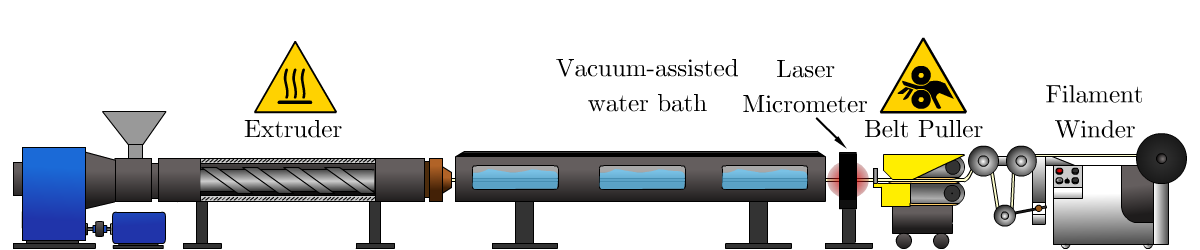
\includegraphics[width=\linewidth]{Extrusion_line}
	\caption{Extrusion line setup} \label{fig:extrLine}
\end{figure}
\pagebreak

\section{Sample Preparation}

As explained in Chapter \ref{ch:oocrit}, the OOC requires mechanical tests to obtain the multiple tensorial components of the mathematical function that describes part failure. Table \ref{tab:testsum} summarizes the tests required.
\begin{table} [h]
\centering
\caption{Mechanical tests required for the OOC}
\begin{tabular}{ c c } 
	\toprule
	\textbf{Mechanical Test} & \textbf{OOC parameters obtained} \\
	\midrule
	Tensile           &   $X_t$, $Y_t$\\
	Compressive       &   $X_c$, $Y_c$\\
	Torsion           &   $S$, $S_{45p}$ , $S_{45n}$\\
	Combined loading  &   $\mu^{1112}$ , $\mu^{2212}$\\
 	\bottomrule
\end{tabular}
\label{tab:testsum}
\end{table}

Given that at the moment of this writing AM testing standards are still in development, custom specimen geometries had to be created in order to test certain loading conditions. Additionally, some bead orientations required are difficult or impossible to reproduce through \emph{2.5-D} FFF. Therefore, the use of a customized robotic, off-axis FFF printer was necessary. This section will detail the coupon geometries used to perform all the mechanical tests described in Table \ref{tab:testsum}, as well as the printing equipment, and toolpath considerations necessary to properly arrange the printed beads in the desired orientation for each condition. 

\subsection{Printing Equipment}
Specimens were produced using either a commercially available desktop FFF printer (Lulzbot TAZ5, USA), or a customized 6-axis robotic printing solution whenever the bead orientation was hard to achieve using a \emph{2.5-D} printer. The robotic printer, developed in the Polymer Engineering Center and nicknamed \emph{Otto} \cite{VanHulle2017}, was based on a 6-axis robot (ABB IRB-120, Switzerland) and fitted with a stationary printhead mounted on an aluminum frame, chosen to be the same extruder from the traditional printer (LulzBot TAZ Single Extruder Tool Head v2, 0.5 mm nozzle, USA) to minimize machine influence on the results. The printing equipment can be seen in Figure \ref{fig:PrintEquip}. 
\begin{figure}[h]
	\center
	\subfloat[TAZ 5 Printer \cite{Lulzbot2018}\label{fig:taz5}]{%
		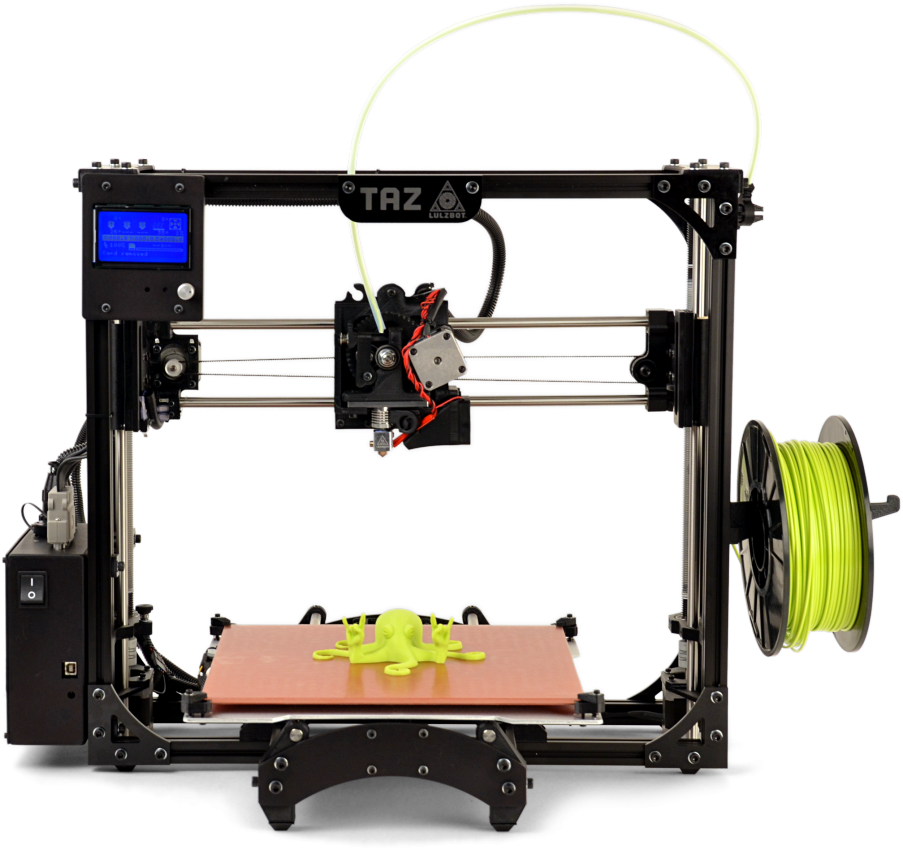
\includegraphics[height=6cm, keepaspectratio]{TAZ_5}
	}
	\hfill
	\subfloat[6-axis robotic printer: \emph{Otto}\label{fig:Otto}]{%
		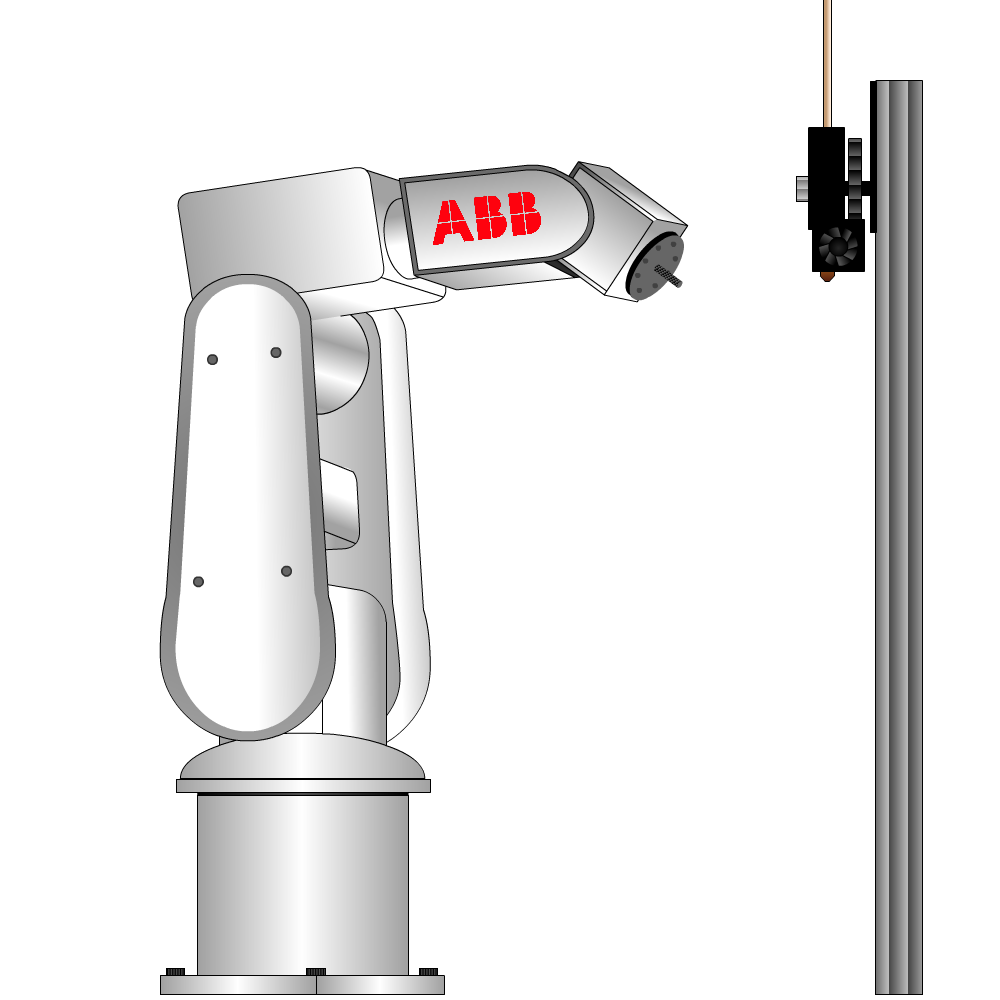
\includegraphics[height=6cm, keepaspectratio]{Otto}
	}
	\caption{Printing equipment} \label{fig:PrintEquip}
\end{figure}

\subsection{Tensile Tests}
Tensile coupons were manufactured on the TAZ5, with bead orientations of 0$^\circ$ and 90$^\circ$ with respect to the load direction in order to test $X_t$ and $Y_t$ respectively. The chosen geometry was the ASTM D-638 Type I coupon \cite{ASTMD638} which can be seen in Figure \ref{fig:db}. The toolpath required to produce these samples was developed through \emph{SciSlice}, a customized slicing engine created in the Polymer Engineering Center that allows layer-by-layer and part-by-part controls of crucial process parameters \textemdash such as the bead orientation \textemdash making it ideal for research in the field of FFF \cite{VanHulle2017a}.

\begin{figure}[h]
	\center
	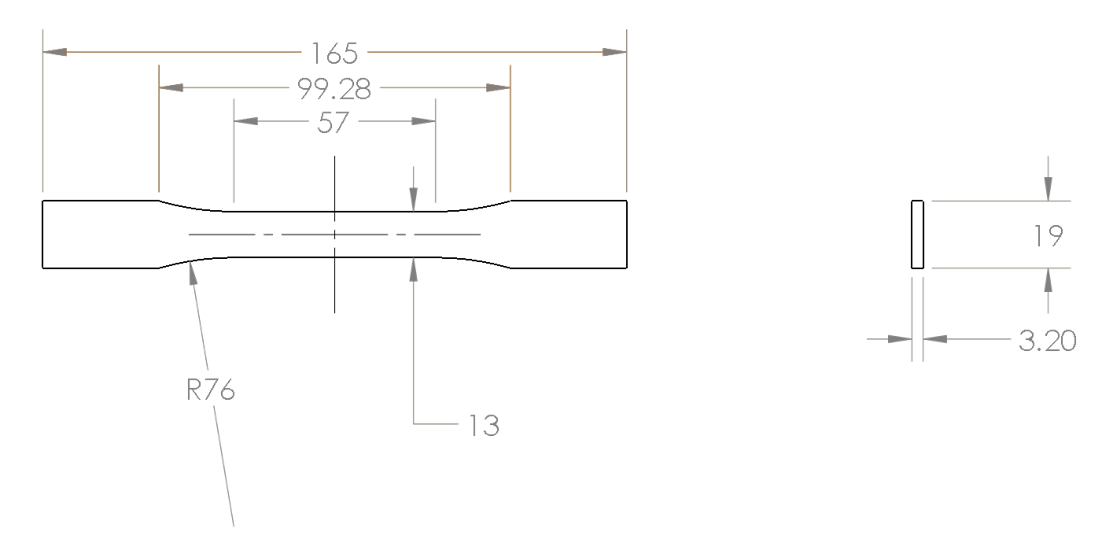
\includegraphics[width=0.95\linewidth, keepaspectratio]{typeIDB}
	\caption{ASTM D-638 Type I coupon} \label{fig:db}
\end{figure}

In order to minimize stress concentrators due to printing discontinuities, the 0$^\circ$ specimens were printed using 13 shells. This produced a continuous toolpath with beads oriented in the loading direction at the neck section of the specimen. No shells were added to the 90$^\circ$ samples. Refer to Figure \ref{fig:090db} for a visual representation of the coupons. 

\begin{figure}[h]
	\center
	
\includegraphics[width=0.8\linewidth, keepaspectratio]{090db}
	\caption{Toolpath considerations for the tensile coupons} \label{fig:090db}
\end{figure}

\subsection{Compressive Tests}

\begin{figure}[h]
	\center
	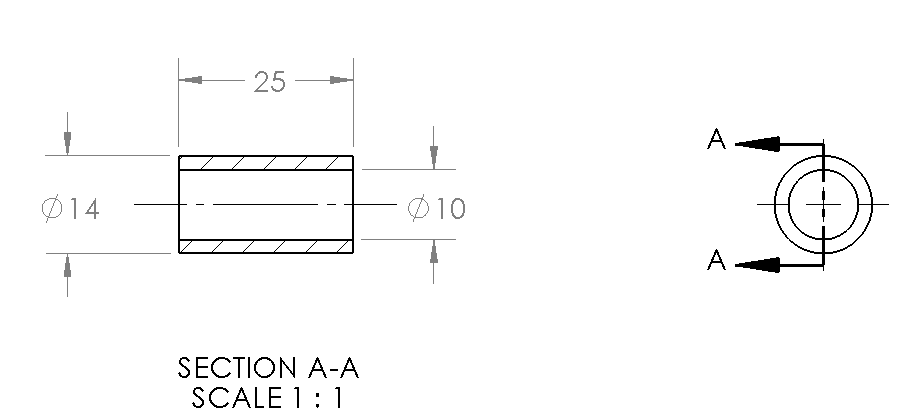
\includegraphics[height=6cm, keepaspectratio]{compres}
	\caption{Compression specimen geometry} \label{fig:comp}
\end{figure}
\subsection{Torsion and Combined Loading Tests}
\begin{figure}[h]
	\center
	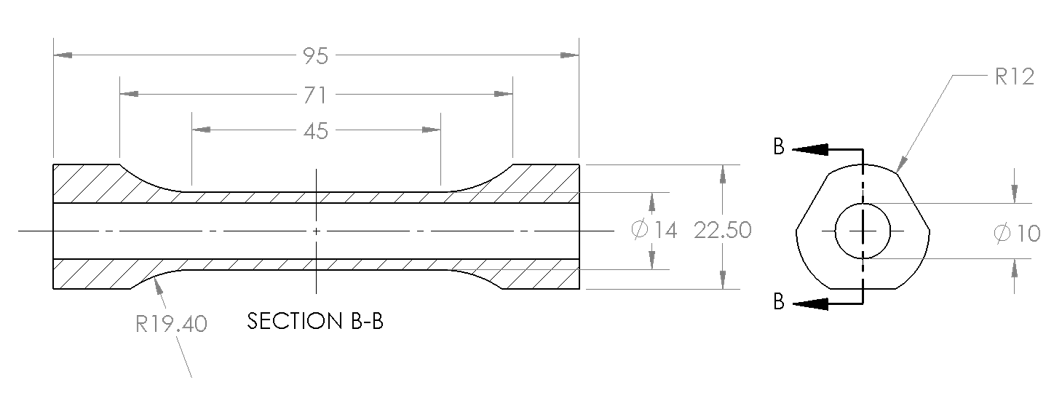
\includegraphics[width=\linewidth, keepaspectratio]{torsion}
	\caption{Torsion specimen geometry} \label{fig:tors}
\end{figure}

\section{Mechanical Testing}
% Nomenclature introduced in this chapter:
\nomenclature[A]{ABS}{Acrylonitrile Butadiene Styrene}% 

% Symbols introduced in this chapter:
%\nomenclature[S]{$X_t$}{Tensile strength in the 1-1 direction \nomunit{$MPa$}}
\end{document}